\section{Key Concepts}

The topologygenerator is a tool for building a custom output file format out of a given network topology. The key concepts in this tool are the followings:
\begin{itemize}
\item Provider \\
Will be in charge of everything which is concerned to the network topology, meanning that it will have to provide information about it's elements, how they are connected between each other, general properties of each of the elements, etc., as well as has the ability to change it's content, for example adding new elements to the network, creating new connections, deleting elements, etc.
\item NetworkTopology \\
Is an abastract representation of the network which will be build by several requests to the provider.
\item Builder \\
Builders will know how to create from a network topology the desired output. For each type of element in the network (for example host, link, device), we will have a builder.\\
This element is easily implemented thanks to the network topology explained above, since this abstraction allow us to decouple from the real provider (it wouldn't be the same to build an element if the provider is Onos or OpenDayLight, since the way of getting the information from the element varies depending on the controller). \\
\item Output \\
Is what we are seeking, our main objective. This output can be either a file or multiple files, and will be generated by either one or multiple builders.
\end{itemize}

Understood the key concepts, let's understand how this elements relates one with each other with some examples of use. We will first start focusing in an abstract example, where we just have one provider and N type's of elements in the network as showed in the next image:

\begin{figure}[H]
\centering
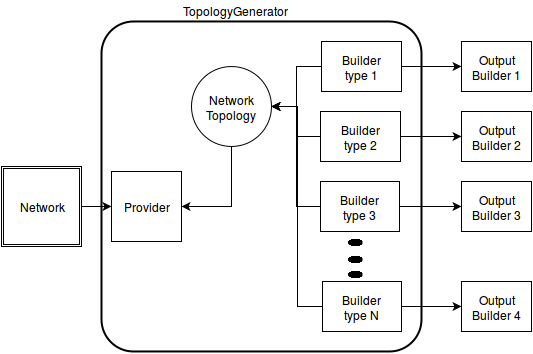
\includegraphics[width=\textwidth]{images/topologygenerator/topologygenerator_abstract_multiple.png}
\caption{Abstract interaction of elements with multiple outputs}
\end{figure}

In this image we can see how the elements explanied above interact. The provider will communicate with the real network, in the image above the real network is represented as the network which is outside the topology generator, to get all the information necessary in order to create the network topology representation. This comunication can either happen locally or remotely as we will see in one of the followings examples.\\
Once the representation is created, the builders are called to generate the output. In this example, we consider having N different types of elements in the network topology, which make us to have N different types of builders (1 per each type). Just to remark what was explained about the output, we are showing an example where we have one output per builder. This is not necessary the only case, as we can see in this other example: 

\begin{figure}[H]
\centering
\includegraphics[width=\textwidth]{images/topologygenerator/topologygenerator_abstract_single.png}
\caption{Abstract interaction of elements with single output}
\end{figure}

As we can see in this case, the logic of joining all the outputs from each of the builder's type is made by a new builder called TopologyBuilder, which is the one who finally generate's the desired output.\\

Let's consider now a concrete example where we want to obtain a network from either ONOS or OpenDayLight controller, and then create a DEVS's model for running simulations. We will assume that we are interested in hosts, devices and links of the network, meaning that we will consider only three types of elements. \\
In this example, we will need to have two providers, one per each controller, three builders, one per each type, and one more builder which will have the logic of joining all the output's provided to generate one common output, the topology.pdm, as show next:

\begin{figure}[H]
\centering
\includegraphics[width=\textwidth]{images/topologygenerator/controller_example.png}
\caption{Controller's example}
\end{figure}

Each of the providers in the image above, will have the knowledge to communicate with it's corresponding controller. In this example, the OnosProvider will encapsulate the logic to communicate with the Api Rest from the Onos controller, meanwhile the OpenDayLightProvider will do the same for the OpenDayLight controller.\\
The interaction with the controller can be either locally, for example this can happens if the controller is set up in the same machine where the topologygenerator is running, or remotely, for example if the controller is set up in a different machine and the comunication is made via http. How to implement both possibilities will be further explained in the next section.\\
The output generated is a pdm which can be interpretated by the DEVS simulator.\\

What happen if we do not have a real network?, What if we have a representation of a network in a programming language, for example Ruby, and we want to create from this network a simulation to test properties?. Then we can use the topologygenerator as follow in the next image:

\begin{figure}[H]
\centering
\includegraphics[width=\textwidth]{images/topologygenerator/ruby_provider.png}
\caption{Ruby as provider and DEVS as output}
\end{figure}
 
This image shows how it's just a question of creating a new provider, in this case the ruby provider, which will be in charge of having the knowledge of how to make the request to the script to obtain all the necessary information in order to create the network topology representation. Since we still want to create a simulation, the builders and the output is still the same. \\

In this previous example we show a powerful characteristic of the tool, which is that providers and builders are not related at all, meaning that changing a provider does not imply to change builders. This characteristic allow us then to create as much providers and builders as we want, and to connect them independently each other to generate as many desired output as we may want. \\

What would happend if we want to try out our custom topology written in Ruby, and test it in an Onos enviorment?, How could we manage to do this?.\\
In this example we would like to have our ruby provider, as in the previous case, and builders that generates request to the ONOS Api as show in the following image:

\begin{figure}[H]
\centering
\includegraphics[width=\textwidth]{images/topologygenerator/onos_builder.png}
\caption{Ruby as provider and ONOS as output}
\end{figure}

Each of the builder's in this case will generate requests to the ONOS Api that will create each of the elements in the SDN enviorment (this is a good example of the capability of SDN, since the enviorment allow us to create elements in the network). \\
In this example, it's important to notice how malleable and easy results to change ONOS, which was though as a provider in previous examples, to a desired output.\\

With the examples showed, we have a good understanding in the power of the tool and how it is supposed to be used. In the following section we will provide a tutorial for using the topologygenerator, and we will implement some of the examples that we have shown until now.

\section{Tutorial}

The topology can be retrieved from a custom file written in ruby by the user, or from an SDN controller (by specifying the API uri). The ONOS controller is currently supported, while the API for OpenDayLight is in progress. When building your output, you have to write a module that describes how to each class defined in the network topology. The topologygenerator gem will then use the defined modules to generate the output desired. You can see examples of how to use this gem in the public github webpage.

\section{Implementation}

\section{Limits}

\section{Future work}